\documentclass[letterpaper]{article}
\usepackage[submission]{aaai2027}
\usepackage{caption}
\usepackage{amsmath,amssymb,booktabs,graphicx,array}
\usepackage{natbib}
\nocopyright
\newcommand{\pp}{\,\mathrm{pp}}

\title{Supplementary Material: Auditing Selection Purity and Transfer Utility under
Joint Model and Data Heterogeneity}
\author{Anonymous Authors}
\affiliations{Anonymous Affiliation}

\begin{document}
\maketitle
\setlength{\emergencystretch}{1em}

\section{Scope}
This supplement retains local-adaptation and natural weak-label evidence that
bounds, but does not add server endpoints to, the main study.  We preserve the
stated development-only, post-observation, and reused-test evidence labels;
relocation outside the main-paper page limit does not upgrade them.

\section{Closest-Work Boundary}
Table~\ref{tab:closest-boundary} states the nearest-method boundary without
claiming a new optimizer or native-setting dominance.
\begin{table*}[t]
\centering
\small
\setlength{\tabcolsep}{3pt}
\begin{tabular}{>{\raggedright\arraybackslash}p{.18\textwidth}
                >{\raggedright\arraybackslash}p{.25\textwidth}
                >{\raggedright\arraybackslash}p{.48\textwidth}}
\toprule
Work & Main focus & Boundary relative to this audit\\
\midrule
Selective-FD \cite{shao2024selectivefd} & Filters misleading client-side
distillation signals & Does not run four contaminated-client arms alongside
matched-\(K\) and maximum-purity controls.\\
FedID \cite{ma2023fedid} & Interactive distillation for pretrained language
models in federated settings & Studies heterogeneous federated distillation
without auditing clean/conflict/off-task purity against server utility.\\
FedHDS \cite{qin2025fedhds} & Representative data selection for federated LLM
instruction tuning & Addresses data-efficient local tuning, whereas our
selection is an audit intervention on transferred canonical probabilities.\\
FedFD \cite{li2025fedfd} & Alignment for unstable heterogeneous logit
ensembles & Establishes that heterogeneous logit ensembles can fail; our
contribution is evidence-labelled failure analysis under internal
contamination.\\
\bottomrule
\end{tabular}
\caption{Closest-work boundary. The paper claims a narrow audit contribution,
not a new optimizer or dominance over these methods in their native settings.}
\label{tab:closest-boundary}
\end{table*}

\section{Complete Legacy Server Endpoints}
Table~\ref{tab:legacy-endpoints} preserves the task-specific discovery
endpoints that contextualize the main audit.
\begin{table*}[t]
\centering
\small
\setlength{\tabcolsep}{3pt}
\begin{tabular}{llccc}
\toprule
Task & Method & Accuracy & Macro-F1 & Score ECE\\
\midrule
AG News & Anchor-only & \(84.34\pm0.62\) & 84.28 & 0.054\\
AG News & Routed & \(83.78\pm0.54\) & 83.67 & 0.016\\
TREC & Anchor-only & \(80.72\pm1.41\) & 77.65 & 0.068\\
TREC & Routed & \(81.12\pm0.67\) & 78.38 & 0.031\\
\midrule
TREC post & Anchor-only & \(81.76\pm2.01\) & 78.39 & 0.060\\
TREC post & Clean uniform & \(81.56\pm1.55\) & 79.01 & 0.035\\
TREC post & Severe uniform & \(83.14\pm0.77\) & 80.80 & 0.099\\
TREC post & Severe routed & \(81.72\pm1.38\) & 79.43 & 0.039\\
\bottomrule
\end{tabular}
\caption{Verified AG News and TREC server endpoints retained from the discovery
stages. Accuracy is mean \(\pm\) SD; macro-F1 and score ECE are seed means.
TREC post rows reuse the already accessed test with ten new seeds.}
\label{tab:legacy-endpoints}
\end{table*}

\section{Full Server Configuration}
All server audits use Qwen2.5-0.5B, SmolLM2-360M, and TinyLlama-1.1B clients
with a Qwen2.5-1.5B server.  LoRA targets query/value projections with rank 4,
scale 8, and zero dropout.  Each run uses two rounds, 40 client and 40 server
steps per round, batch size 8, client learning rate \(10^{-3}\), server learning
rate \(10^{-4}\), anchor weight 1, and distillation weight 0.25.  Clients
transmit the uniform mean of canonical verbalizer probabilities; no model
parameter is aggregated across architectures.

The four arms are: A, public-anchor-only server training; B, uniform transfer
from clean clients; C, uniform transfer from the joint severe mixture; and D,
the complete severe routed intervention.  AG News uses 256 anchors, 800
development rows, and the 7,600-row official test.  TREC uses 72 anchors, 72
development questions, three 120-question client pools, and the 500-question
official test.  IMDb uses 128 anchors, 1,000 development reviews, three
256-example client pools, and all 25,000 official test reviews.  Each severe
IMDb client contains 103 clean, 102 conflict, and 51 off-task examples.

The IMDb secondary addendum fixes \(K=128\), 64 rows per claimed label, the
severe source mixture, optimizer steps, and all server settings.  Random-\(K\)
samples only from target-eligible rows; routed-\(K\) uses the frozen routing
order; maximum-purity-\(K\) contains 103 clean and 25 conflict rows.  The last
arm is an audit-only attainable upper control, not a clean-only method.

\section{Post-hoc IMDb Selector-Component Diagnostic}
After the IMDb primary and matched-\(K\) results were observed, we ran a
post-hoc reused-test diagnostic that replaces the full routed-\(K\) score with
one component at a time while preserving \(K=128\), 64 examples per claimed
label, the severe mixture, models, anchors, optimizer settings, and server
training budget.  The new 30 records cover ten seeds and three arms:
gradient-only, loss-only, and margin-only.  The existing verified
routed-\(K\) matched-size records serve as the full-router reference.

Mean accuracies are 91.46\% for full routed-\(K\), 91.30\% for gradient-only,
91.50\% for loss-only, and 91.36\% for margin-only.  The three post-hoc
paired contrasts use one Holm family: full-minus-gradient is \(+0.16\pp\)
(95\% CI \([+0.00,+0.32]\), Holm \(p=.135\)); full-minus-loss is
\(-0.04\pp\) (\([-0.17,+0.09]\), Holm \(p=.505\)); and full-minus-margin is
\(+0.10\pp\) (\([-0.00,+0.21]\), Holm \(p=.135\)).  Audited clean fractions
are 71.0\%, 59.4\%, 67.3\%, and 71.6\%, respectively.  Thus the diagnostic
does not isolate a statistically detectable single-component replacement gap
after multiplicity correction, and it does not change the primary IMDb gate or
the matched-\(K\) secondary family.

\section{Compatible Co-Teaching Control}
We compare naive LoRA to two-peer Co-Teaching on frozen AG News development
mixtures.  Co-Teaching receives the true total contamination fraction as its
forget rate, and peer probabilities are ensembled at evaluation.  This is an
oracle-rate compatible-model control, not a heterogeneous server baseline.

\begin{table}[ht]
\centering
\small
\begin{tabular}{lrr}
\toprule
Client & Conflict 40\% & Joint 40\%/20\%\\
\midrule
Qwen & 59.12 / 60.92 (+1.79) & 53.71 / 54.50 (+0.79)\\
SmolLM2 & 65.83 / 68.46 (+2.63) & 48.00 / 47.37 (-0.63)\\
TinyLlama & 59.25 / 68.54 (+9.29) & 54.92 / 37.25 (-17.67)\\
\bottomrule
\end{tabular}
\caption{Three-seed AG News development accuracy: naive / Co-Teaching
(percentage-point change).}
\end{table}

No contrast survives Holm correction over the six contaminated comparisons
(all adjusted $p=1.0$), and seed-wise effects change sign in five settings.
The jointly contaminated TinyLlama setting also lies outside Co-Teaching's
original finite-label-noise scope.  Concurrently scheduled wall-time ratios of
$2.84$--$9.32\times$ are environment-specific diagnostics.

\section{Natural Weak Labels}
Hausa and Yoruba topic-classification corpora provide naturally occurring weak
labels paired with released clean annotations \cite{hedderich2020transfer}.
The weak/clean disagreement
rates are 50.37\% for 2,045 Hausa training headlines and 33.28\% for 1,340
Yoruba headlines.  The corpus-level rate is supplied as Co-Teaching's oracle
forget rate; per-example clean labels never enter model input, gradients, or
selection scores.  Only the clean development splits are evaluated.

Across three seeds, Hausa naive/Co-Teaching accuracies are 44.94/33.33 for
Qwen, 45.29/28.16 for SmolLM2, and 47.82/28.74 for TinyLlama, giving changes of
$-11.61$, $-17.13$, and $-19.08\pp$.  The frozen gate fails and the clean test
split remains unused.  Yoruba changes are $+0.53$, $+2.65$, and $-4.23\pp$;
all intervals cross zero, so its gate also fails and its test split is not
evaluated.  Co-Teaching raises Yoruba selected clean-label agreement from
66.72\% to 78.2\%--80.6\% without a reliable accuracy gain.  This is a local
counterexample to treating selection purity as sufficient for utility, not a
server-transfer result.  In Hausa, weak labels match the released clean labels
on 49.63\% of training examples, while selected agreement ranges from
45.3\%--50.9\%.  Its concurrently scheduled Co-Teaching runs cost
\(1.69\)--\(1.80\times\) the naive wall time; these are environment-specific
diagnostics.

\section{Open-Answer Teacher Ranking}
GSM8K supplies target questions and SQuAD supplies off-task QA
\cite{cobbe2021gsm8k,rajpurkar2016squad}.  A teacher is
trained only on the public anchor and ranks supplied numerical answers by
token-normalized answer loss.  For a supplied pair
\(z=(x,\widetilde y)\), its score is
\[
s_T(z)=-|\widetilde y|^{-1}\log p_{f_T}(\widetilde y\mid x).
\]
After a numerical-interface check, the client retains the \(K_{\mathrm{local}}\) highest-score
examples and performs the same optimizer-step budget as the unfiltered arm.
No teacher parameter, hidden state, validation label, or test example enters
client training.  On the official GSM8K test, Qwen severe-mixture
exact match rises from 3.49\% EM to 6.82\% ($+3.34\pp$); clean exact match rises
from 6.62\% to 7.91\%.  This supports a narrow local Qwen endpoint, not
beneficial federated transfer.  The client families are documented in their
model reports \cite{qwen2025technical,benallal2025smollm2,zhang2024tinyllama}.

\begin{table}[ht]
\centering
\small
\begin{tabular}{llrrr}
\toprule
Client & Condition & Naive & Teacher & Gain\\
\midrule
SmolLM2 & clean  & 4.55 & 4.90 & +0.35\\
SmolLM2 & severe & 2.58 & 4.17 & +1.59\\
TinyLlama & clean  & 3.66 & 4.25 & +0.58\\
TinyLlama & severe & 1.42 & 3.44 & +2.02\\
\bottomrule
\end{tabular}
\caption{Post-observation non-Qwen GSM8K extension.  The two severe hypotheses
form a Holm family.}
\end{table}

All six seed-level severe differences are positive, and both clean safety
gates hold.  Nevertheless, both severe confidence intervals cross zero and
both Holm-adjusted tests have \(p=0.0714\); the declared cross-family claim fails.
On development data, teacher ranking exceeds matched numeric-random and client
small-loss selectors by \(+0.78/+0.98\pp\) for SmolLM2 and
\(+1.56/+1.50\pp\) for TinyLlama.  These post-hoc controls cannot repair the
failed official cross-family gate.

\begin{table*}[t]
\centering
\small
\begin{tabular}{lrrrrrr}
\toprule
& \multicolumn{2}{c}{Clean} & \multicolumn{2}{c}{Medium (20/10)}
& \multicolumn{2}{c}{Severe (40/20)}\\
Client & Naive & Teacher & Naive & Teacher & Naive & Teacher\\
\midrule
Qwen & 6.38 & 6.84 (+0.46) & 5.24 & 7.85 (+2.60) & 1.69 & 5.76 (+4.07)\\
SmolLM2 & 3.68 & 2.80 (-0.88) & 2.15 & 3.39 (+1.24) & 1.46 & 2.47 (+1.01)\\
TinyLlama & 2.99 & 2.93 (-0.07) & 2.02 & 2.44 (+0.42) & 1.07 & 1.73 (+0.65)\\
\bottomrule
\end{tabular}
\caption{Disjoint 1,024-example post-primary severity curve.  Values are mean
exact match; parentheses show teacher-minus-naive percentage-point changes.}
\end{table*}

The descriptive curve gate passes, but none of nine family-by-severity tests
survives joint Holm correction.  Matched development selectors support a
teacher-signal interpretation without repairing the failed official
cross-family gate.  A matched 64-question diagnostic gives $1.52\times$ and
$1.58\times$ wall-time ratios for SmolLM2 and TinyLlama; serial scoring of 256
candidates takes approximately 8.1 seconds and peaks at 5.57 GiB allocated GPU
memory on the recorded host.

\begin{figure*}[t]
\centering
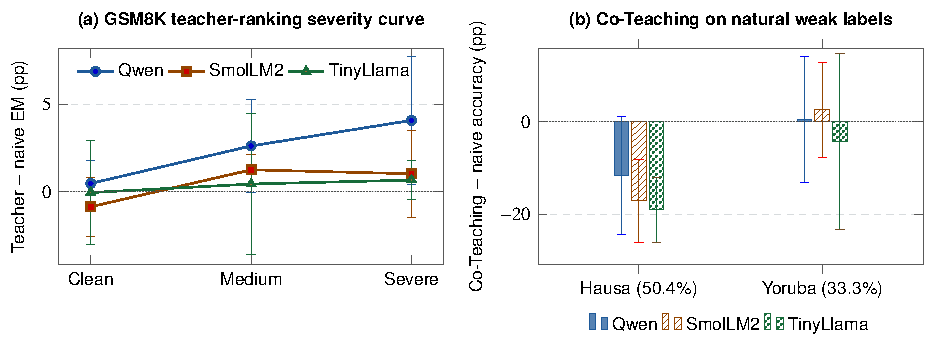
\includegraphics[width=0.94\textwidth]{figures/evidence.pdf}
\caption{Paired mean changes with descriptive 95\% Student-$t$ intervals over
three seeds.  Left: GSM8K teacher-ranking severity curve.  Right: Hausa and
Yoruba oracle-rate Co-Teaching effects.  Intervals describe seed variation;
the pre-specified gates described above remain failed.}
\end{figure*}

\section{Artifact Reconstruction and Failure Policy}
The reconstruction path is content addressed rather than inferred from a
paper table.  Each server study has a frozen protocol and manifest recording
the task specifications, source-file hashes, model-weight hashes, data
partitions, seed set, method matrix, and analysis rule.  Protocol histories
also retain pre-evaluation instrumentation repairs instead of silently
rewriting their chronology.  Development and official evaluation use separate
phase directories, seed ranges, and output names.  Where a development phase
must not access a test split, a nonexistent sentinel is part of the verifier's
contract.  Thus a development artifact cannot be relabelled as an official
record merely by moving or renaming it.

Reconstruction begins from the per-run JSON records, not from rounded values
in the manuscript.  A phase verifier checks the expected seed--method
Cartesian product, record identities, frozen protocol and configuration
fields, evaluation counts, finite metrics, and method-specific invariants.
The IMDb matched-size analysis additionally verifies its fixed cardinality,
claimed-label quotas, mixture identity, and a separate conditional
implementation relationship receipt for the routed original and routed-\(K\)
arms.  The paper-asset generator first requires the exact complete matrices and
positive verifier certificates.  Only then does it load the raw JSON, recompute
arm means and sample standard deviations, paired differences and Student-$t$
intervals, the frozen paired tests and Holm adjustment, exact sign-flip
sensitivity where declared, and audited selection composition.  A single
machine-readable statistics file is then used to emit the TeX macros, tables,
English results block, and vector figure.  These files are built in a temporary
staging directory and replace the published asset set only after figure
compilation succeeds.

The routed relationship verifier was corrected after all 70 IMDb official
records already existed.  The verifier frozen at official start
(\texttt{2c8678f7...}) incorrectly required unconditional whole-record
identity, even when the original conditional gate retained all 256 examples and
the matched protocol deliberately forced \(K=128\).  The repaired verifier
(\texttt{5518b177...}) checks exact identity only before a local gate fork,
records the original gate decision as the only authorized first divergence, and
then checks each arm's frozen branch invariants.  It partitions the 60
client-rounds into 55 exact pre-fork triggered rounds, four first authorized
gate divergences, and one post-local-fork round that is not
relationship-eligible; six of ten seed trajectories are fully identical.  No
raw JSON, seed, arm, metric, statistic, protocol, or runner changed, and this
receipt is separate from the three scientific IMDb gate clauses.

Failure is therefore explicit and fail-closed.  A missing or extra record, an
identity mismatch, a non-finite metric, a verifier rejection, a failed
conditional relationship receipt, or failed figure compilation prevents
publication of a new asset set unless a verifier defect is disclosed, patched,
and regression-tested without changing records or reported statistics.  Aborted
and invalidated attempts may remain as timestamped failure logs for audit, but
they are not members of the verified matrix and cannot enter a summary.
Partial official results may be observed solely to diagnose process health;
they do not authorize seed changes, stopping, hyperparameter updates, new
contrasts, or manuscript numbers.  Official claims are generated only after the
full frozen matrix passes its verifier.  These checks establish the reported
artifact path; they are not a claim that every legacy or optional test in the
broader repository succeeds in the present environment.

\section{Evidence Boundary}
The GSM8K Qwen result is the only positive official local endpoint in this
supplement.  The non-Qwen extension follows observation of the Qwen phase on
the same official test, the severity curve is post-primary, and both natural
weak-label studies are development-only.  None of these studies establishes a
general federated algorithm, privacy property, or task-population effect.

\begingroup
\small
\bibliography{references}
\endgroup

\end{document}
